% Copyright 2026 Sreeram Anil
% SPDX-License-Identifier: CC-BY-4.0
\chapter{Unscented Rauch--Tung--Striebel smoother (URTS)}
\label{ch:urts}

\section*{At a glance}
\begin{tabular}{@{}l>{\raggedright\arraybackslash}p{0.76\textwidth}@{}}
Family & Smoothing (offline / fixed interval) \\
Header & \texttt{include/estkit/smoothers/urts.hpp} \\
Registered name & \texttt{URTS} \\
State dimension & $n_x=4$, $2n_x+1=9$ sigma points \\
Cost per step & $\mathcal{O}(n_x^3)$ plus $3n_x+1$ extra model evaluations; \SI{2.50}{\micro\second}/step measured \\
Memory & $N\left(2n_x+3n_x^2+n_u\right)$ reals; \SI{12.5}{\mega\byte} for $N=20\,100$ \\
Primary references & \cite{sarkka2008urts,sarkka2013,rauch1965rts,julier2004unscented} \\
\end{tabular}

\section{Motivation and aerospace/BMS relevance}
The extended RTS smoother of Chapter~\ref{ch:erts} inherits two things from its forward EKF: the
trajectory it refines, and the Jacobian $\mF_k$ that defines its gain.  Both are weaknesses.  The
first is fundamental --- the results of Chapter~\ref{ch:erts} show that where the forward EKF fails
(the \texttt{combined} scenario) the smoother fails with it.  The second is the usual linearisation
error: the cell model's hysteresis state evolves through
$h_{k+1}=A_h h_k+(A_h-1)\sgn(i)$ with $A_h=\exp(-|\eta i\gamma\dt/(3600Q)|)$, a genuinely nonlinear
map whose Jacobian is a poor description when the current changes sign, and the OCV is a table whose
slope changes by a factor of three across the SOC range.

Särkkä's unscented RTS smoother~\cite{sarkka2008urts} removes both at once.  The observation behind
it is that the RTS gain
\begin{equation}
\mG_k=\mP^+_k\mF_k^\T\left(\mP^-_{k+1}\right)\inv
\label{eq:urts-motiv}
\end{equation}
does not really need a Jacobian: $\mP^+_k\mF_k^\T$ is nothing but the cross-covariance
$\operatorname{cov}\!\left(\vx_k,\vx_{k+1}\mid\vy_{0:k}\right)$, and a cross-covariance is exactly
the kind of quantity the unscented transform computes directly and accurately.  Replacing the
Jacobian product by the sigma-point estimate makes the smoother second-order accurate for any smooth
$f$, and it removes the need to differentiate the model at all.

For post-flight battery work the practical consequence is the one measured in
Section~\ref{sec:urts-results}: on the hardest scenario in the benchmark URTS produces an SOC
trajectory that is fourteen times more accurate than the extended smoother's, purely because its
forward pass is a UKF and its backward gain does not rely on a linearisation of the hysteresis
dynamics.  For a ground station that has to produce a defensible reconstruction from a flight in
which something went wrong --- a cold soak, a mis-calibrated shunt, a degraded cell --- that
difference decides whether the reconstruction is usable.

\section{Problem statement and assumptions}
The problem is that of Chapter~\ref{ch:erts}: given the whole record $\vy_{0:N-1}$ of the system
\eqref{eq:rts-f}--\eqref{eq:rts-h}, compute $(\xhat^s_k,\mP^s_k)$ for every $k$.  What changes is the
approximation used for the joint density of $(\vx_k,\vx_{k+1})$.

\begin{assumption}[Unscented joint approximation]\label{as:urts-joint}
The joint density of $(\vx_k,\vx_{k+1})$ given $\vy_{0:k}$ is Gaussian with the mean and covariance
produced by the scaled unscented transform of $f$ applied to $\N{\xplus_k}{\mP^+_k}$.  In
particular the cross-covariance is the weighted empirical cross-covariance \eqref{eq:urts-C}, not
$\mP^+_k\mF_k^\T$.
\end{assumption}

\begin{assumption}[Moment adequacy]
The filtering and smoothing densities are adequately described by two moments, and $f$ is twice
differentiable so that the unscented transform is exact to second order~\cite{julier2004unscented}.
\end{assumption}

\section{Derivation}

\subsection{The cross-covariance form of the RTS gain}
Return to the joint density \eqref{eq:rts-joint} of the previous chapter, written without committing
to a linearisation:
\begin{equation}
\begin{bmatrix}\vx_k\\ \vx_{k+1}\end{bmatrix}\Bigg|\,\vy_{0:k}
\;\approx\;
\N{\begin{bmatrix}\xplus_k\\ \xminus_{k+1}\end{bmatrix}}
 {\begin{bmatrix}\mP^+_k & \mC_k\\ \mC_k^\T & \mP^-_{k+1}\end{bmatrix}},
\qquad
\mC_k=\E{\left(\vx_k-\xplus_k\right)\left(\vx_{k+1}-\xminus_{k+1}\right)^\T\mid\vy_{0:k}} .
\label{eq:urts-joint}
\end{equation}
Gaussian conditioning gives exactly the same structure as before but with the gain expressed through
the cross-covariance:
\begin{equation}
\boxed{\;\mD_k=\mC_k\left(\mP^-_{k+1}\right)\inv\;}
\qquad
\xhat^s_k=\xplus_k+\mD_k\left(\xhat^s_{k+1}-\xminus_{k+1}\right),
\qquad
\mP^s_k=\mP^+_k+\mD_k\left(\mP^s_{k+1}-\mP^-_{k+1}\right)\mD_k^\T .
\label{eq:urts-rec}
\end{equation}
For a linear $f$, $\mC_k=\mP^+_k\mF^\T$ exactly and \eqref{eq:urts-rec} reduces to
\eqref{eq:rts-gain}: the URTS is a strict generalisation of the extended RTS smoother.

\subsection{The sigma-point cross-covariance}
Let $\{\mathcal{X}^{(j)}_k\}_{j=0}^{2n_x}$ be the scaled unscented sigma set of
$\N{\xplus_k}{\mP^+_k}$, with weights $w^{(j)}_m,w^{(j)}_c$ defined as in \eqref{eq:ju-lambda}--\eqref{eq:ju-weights}
but with $n_a$ replaced by $n_x$.  Propagating the set through the dynamics,
\begin{equation}
\mathcal{X}^{(j)}_{k+1|k}=f\!\left(\mathcal{X}^{(j)}_k,\vu_k\right),
\qquad
\xminus_{k+1}=\sum_{j} w^{(j)}_m\,\mathcal{X}^{(j)}_{k+1|k},
\label{eq:urts-prop}
\end{equation}
and the required moments are the weighted empirical ones:
\begin{align}
\mP^-_{k+1}&=\sum_j w^{(j)}_c\left(\mathcal{X}^{(j)}_{k+1|k}-\xminus_{k+1}\right)\left(\cdot\right)^\T+\mQ_k,
\label{eq:urts-P}\\
\mC_k&=\sum_j w^{(j)}_c\left(\mathcal{X}^{(j)}_k-\xplus_k\right)\left(\mathcal{X}^{(j)}_{k+1|k}-\xminus_{k+1}\right)^\T .
\label{eq:urts-C}
\end{align}
Equation~\eqref{eq:urts-C} is Särkkä's key expression~\cite[Eq.~(11)]{sarkka2008urts}: the smoother
gain is obtained from the same nine function evaluations that the forward UKF already needs, with no
derivative and no extra assumption.

\begin{remark}[Why this is better than a Jacobian here]
For the cell model, $\partial f/\partial\vx$ is diagonal, so the extended gain
$\mP^+\mF^\T$ merely rescales the columns of $\mP^+$.  The unscented $\mC_k$ is not constrained to
that structure: when a sigma point straddles a current sign change, its hysteresis coordinate is
propagated through the true, non-differentiable map, and the resulting cross-covariance has
off-diagonal terms the Jacobian form cannot produce.  This is where the accuracy difference on the
hysteresis-dominated scenarios comes from.
\end{remark}

\subsection{Numerical form of the gain}
As in Chapter~\ref{ch:erts} the inverse is avoided: from the symmetry of $\mP^-_{k+1}$,
\begin{equation}
\mD_k^\T=\left(\mP^-_{k+1}\right)\inv\mC_k^\T ,
\label{eq:urts-solve}
\end{equation}
one Cholesky solve per sample.

\section{Algorithm}
\begin{algorithm}[H]
\caption{Unscented RTS smoother --- whole record}
\begin{algorithmic}[1]
\Require $\{i_k,v_k,T_k\}_{k=0}^{N-1}$, model, $\xhat_0,\mP_0$
\State \textbf{Forward pass:} initialise the UKF with $(\xhat_0,\mP_0)$
\For{$k=0,\dots,N-1$}
   \State $\vu_k\gets[i_k,T_k]^\T$
   \If{$k>0$}
      \State regenerate $\{\mathcal{X}^{(j)}\}$ from $(\xplus_{k-1},\mP^+_{k-1})$; propagate by \eqref{eq:urts-prop} with $\vu_{k-1}$
      \State store $\mC_{k-1}$ from \eqref{eq:urts-C}; UKF time update with $\vu_{k-1}$
   \EndIf
   \State store $\xminus_k,\mP^-_k$; UKF measurement update with $y_k=v_k$; store $\xplus_k,\mP^+_k$
\EndFor
\State \textbf{Backward pass:} $\xhat^s_{N-1}\gets\xplus_{N-1}$, $\mP^s_{N-1}\gets\mP^+_{N-1}$
\For{$k=N-2,\dots,0$}
   \State $\mD_k^\T\gets$ \texttt{solve\_spd}$\left(\mP^-_{k+1},\ \mC_k^\T\right)$
   \State $\xhat^s_k\gets\xplus_k+\mD_k(\xhat^s_{k+1}-\xminus_{k+1})$; \quad $\mP^s_k\gets\mP^+_k+\mD_k(\mP^s_{k+1}-\mP^-_{k+1})\mD_k^\T$
   \State symmetrise, project, fall back to $(\xplus_k,\mP^+_k)$ on any non-finite value
\EndFor
\Ensure $\{\xhat^s_k,\mP^s_k\}$; report $\soc^s_k$ and $\hat v_k=h(\xhat^s_k,\vu_k)$
\end{algorithmic}
\end{algorithm}

\section{Application to the battery model}
\texttt{UnscentedRtsSmoother<Model>} instantiates the library's \texttt{Ukf<EcmModel>} as its
forward filter and derives from \texttt{estkit::BatchEstimator}.  The unscented parameters are
$\alpha=0.1$, $\beta=2$, $\kappa=0$, identical to the registered UKF, and $\mQ$, $\mR$ are the
model's own with \texttt{q\_scale}\,$=$\,\texttt{r\_scale}\,$=1$; as for ERTS, using the same tuning
as the corresponding filter makes the comparison in Section~\ref{sec:urts-results} attributable to
smoothing alone.

The cross-covariance \eqref{eq:urts-C} is computed by regenerating the sigma set from
$(\xplus_{k-1},\mP^+_{k-1})$ immediately before the filter's own \texttt{predict()} call.  Because
\texttt{Ukf::sigma\_points()} is deterministic and is called with the same arguments, the set is
bit-identical to the one the filter uses internally; the only cost is one extra unscented
propagation ($2n_x+1=9$ evaluations of $f$) per sample.  Exposing the filter's internal sigma set
instead would halve that cost but would couple the smoother to the filter's internals, which the
generic interface of \texttt{docs/ESTIMATOR\_API.md} deliberately avoids.

As in Chapter~\ref{ch:erts}, the reported \texttt{voltage\_pred} is the smoothed reconstruction
$h(\xhat^s_k,\vu_k)$, not a one-step prediction.

\section{Implementation notes}
Storage is the same $58$ reals per sample as ERTS ($\mC_k$ replaces $\mF_k$), i.e.\
\SI{12.5}{\mega\byte} for the $20\,100$-sample mission.  The measured cost is
\SI{2.50}{\micro\second}/step, $2.8\times$ ERTS and $5.2\times$ the plain EKF; the extra
cost is the additional unscented propagation and the Cholesky factorisation in
\eqref{eq:urts-prop}, which \texttt{cholesky\_safe} regularises with a relative jitter if the
forward covariance loses definiteness.

The backward recursion is guarded exactly as in ERTS: a non-finite gain or a non-finite smoothed
moment causes that sample to fall back to the filtered values.  In the single-precision build the
mission completes with an SOC RMSE of $0.0020$ against $0.0018$ in double precision.  The place
where single precision would eventually bite is \eqref{eq:urts-P}: with $\alpha=0.1$ and $n_x=4$ the
sigma points sit at $0.2\sigma$ and the empirical covariance is a difference of nearly equal terms,
which is the classical argument for a square-root implementation (SR-UKF) in a flight build.

A subtle point worth recording: \eqref{eq:urts-C} must use the sigma set drawn from the
\emph{posterior} $(\xplus_k,\mP^+_k)$, not the one the filter happens to hold after its update.  The
two differ whenever the filter applies a state constraint, and using the wrong set silently biases
the gain.

\section{Benchmark results}
\label{sec:urts-results}
% Copyright 2026 Sreeram Anil
% SPDX-License-Identifier: CC-BY-4.0
\begin{table}[H]\centering\footnotesize\setlength{\tabcolsep}{4pt}
\caption{URTS: cell-level benchmark on the eVTOL mission (mean over seeds; RMSE and max error in \% SOC; $t_\mathrm{conv}$: first time the error stays below 2\,\% for 60\,s, -- = never; EKF reference: steady-state RMSE of the plain EKF on the same data).}\label{tab:cell_URTS}
\begin{tabular}{llrrrrrcrr}\toprule
plant & scenario & RMSE & RMSE$_\mathrm{ss}$ & max & $t_\mathrm{conv}$ [s] & RMSE$_v$ [mV] & div. & EKF ref. & ns/step \\ \midrule
ECM & nominal & 0.13 & 0.04 & 0.31 & 0 & 0.74 & no & 0.05 & 2473 \\
ECM & init\_error & 0.11 & 0.04 & 0.25 & 0 & 0.77 & no & 0.05 & 2478 \\
ECM & current\_bias & 1.09 & 0.41 & 2.33 & 200 & 0.86 & no & 0.61 & 2487 \\
ECM & noise\_step & 0.12 & 0.06 & 0.27 & 0 & 2.21 & no & 0.12 & 2473 \\
ECM & outliers & 0.18 & 0.12 & 0.38 & 0 & 1.61 & no & 0.21 & 2506 \\
ECM & cold & 0.20 & 0.10 & 0.41 & 0 & 1.82 & no & 0.16 & 2486 \\
ECM & hot & 0.08 & 0.02 & 0.22 & 0 & 0.49 & no & 0.03 & 2478 \\
ECM & aged\_cell & 3.70 & 1.68 & 7.63 & 1263 & 9.58 & no & 1.52 & 2474 \\
ECM & param\_mismatch & 1.26 & 1.35 & 1.46 & 0 & 2.25 & no & 1.36 & 2468 \\
ECM & sensor\_dropout & 0.75 & 0.59 & 1.05 & 0 & 1.86 & no & 0.46 & 2476 \\
ECM & preisach & 0.43 & 0.49 & 0.54 & 0 & 2.88 & no & 0.20 & 2479 \\
ECM & combined & 1.50 & 0.67 & 3.22 & 387 & 4.23 & no & 12.44 & 2481 \\
\midrule
SPM & nominal & 3.50 & 3.54 & 3.61 & -- & 2.20 & no & 3.73 & 2339 \\
SPM & init\_error & 4.09 & 4.13 & 4.21 & -- & 0.90 & no & 3.81 & 2351 \\
SPM & current\_bias & 5.14 & 5.95 & 6.82 & -- & 2.67 & no & 5.69 & 2307 \\
SPM & noise\_step & 1.95 & 1.86 & 2.10 & -- & 2.64 & no & 3.30 & 2333 \\
SPM & outliers & 1.37 & 1.43 & 1.51 & 0 & 1.92 & no & 1.99 & 2334 \\
SPM & cold & 9.96 & 10.24 & 10.49 & -- & 4.06 & no & 7.35 & 2340 \\
SPM & hot & 2.02 & 2.09 & 2.19 & -- & 1.11 & no & 2.16 & 2335 \\
SPM & param\_mismatch & 4.57 & 4.65 & 4.75 & -- & 2.00 & no & 3.13 & 2355 \\
SPM & sensor\_dropout & 6.78 & 6.75 & 6.89 & -- & 6.14 & no & 5.31 & 2331 \\
\bottomrule\end{tabular}\end{table}

\begin{figure}[H]\centering
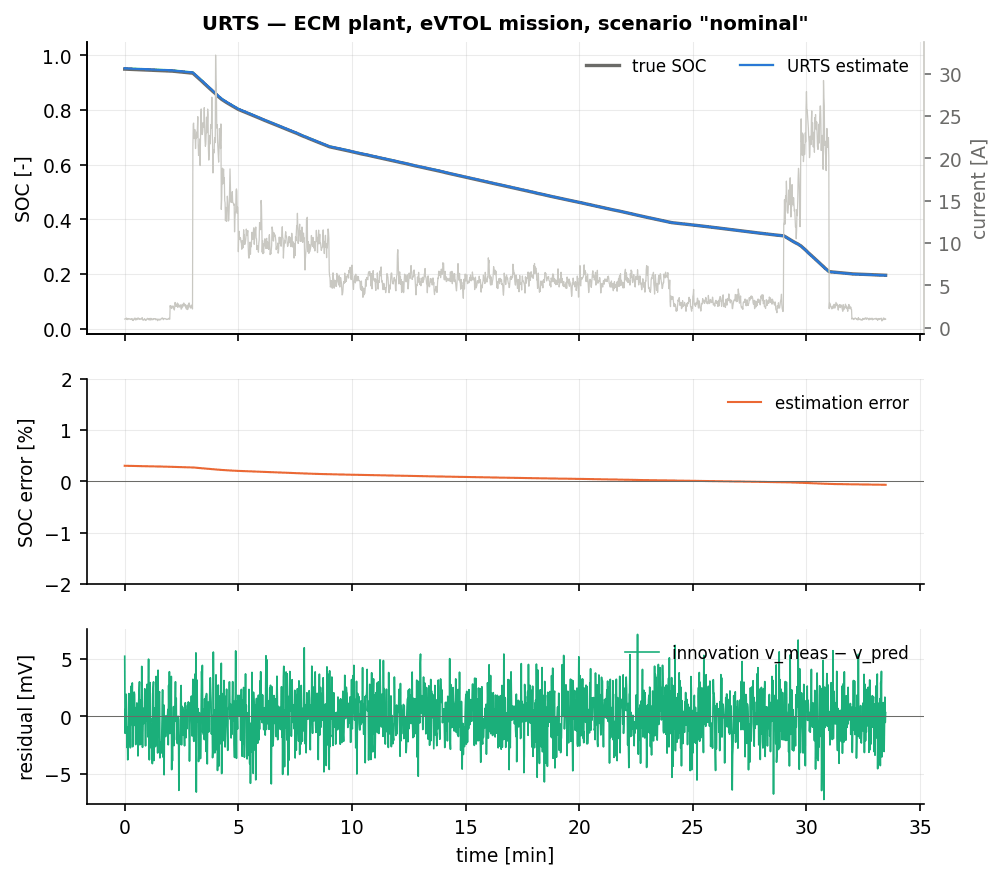
\includegraphics[width=\textwidth]{figures/cell_URTS_nominal.png}
\caption{URTS on the nominal eVTOL mission: true and smoothed SOC (top), estimation error with the $\pm 2\sigma$ band (middle), smoothed voltage residual (bottom).}
\end{figure}
\begin{figure}[H]\centering
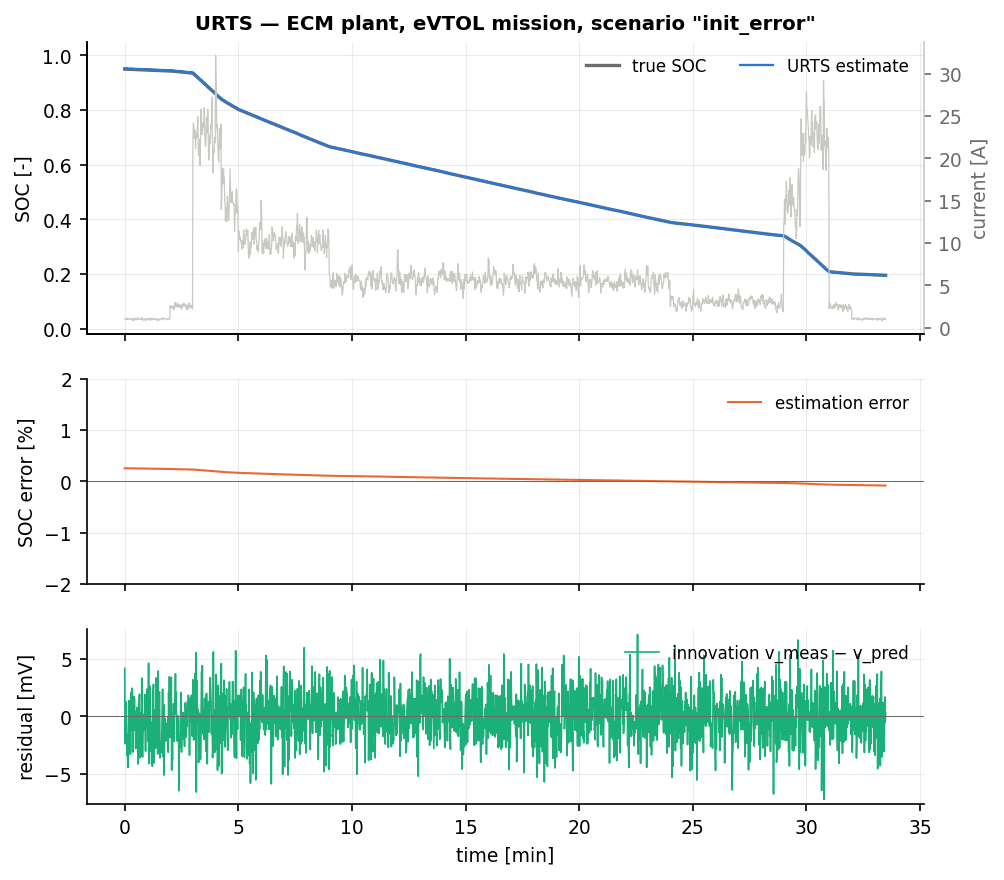
\includegraphics[width=\textwidth]{figures/cell_URTS_init_error.png}
\caption{URTS with a \SI{35}{\percent} initial SOC error.}
\end{figure}

\paragraph{Correct-model diagnostic.}  With an ideal current sensor (no scale-factor error, no
offset --- the only error source in the benchmark that is absent from $\mQ$), the same eVTOL mission
gives an SOC RMSE (mean of three seeds) of $0.00170$ for the EKF and $0.00028$ for both ERTS and
URTS: on this plant, where the dynamics are close enough to linear over one sampling period, the
sigma-point cross-covariance and the Jacobian product agree to within the seed-to-seed scatter.
What \eqref{eq:urts-C} buys here is therefore not accuracy on well-behaved data but robustness ---
see the \texttt{combined} column below --- and the removal of the Jacobian altogether.

\paragraph{Benchmark scenarios.}  All figures are means over three seeds.  On \texttt{nominal} URTS gives $\text{RMSE}=0.0013$,
$\text{RMSE}_\text{ss}=0.0004$, converging at $t=0$ (plain EKF $0.0015/0.0005$, plain UKF
$0.0020/0.0004$).  On \texttt{init\_error} it gives $0.0011/0.0004$, the best run-average figure of
any method in this report, again converging immediately.  Both acceptance criteria are met; no
scenario diverges in any seed.  As explained at length in Chapter~\ref{ch:erts}, the run-average
figure on \texttt{nominal} is dominated by the ramp that the unmodelled \SI{+0.5}{\percent}
current-sensor scale factor imposes on any smoother with a rigid process model.

The decisive column is \texttt{combined} --- a \SI{-25}{\percent} initial SOC error, a
\SI{150}{\milli\ampere} current bias with \SI{+2}{\percent} gain, a \SI{0}{\celsius} ambient and a
\SI{10}{\percent} capacity loss, all at once.  URTS scores $\text{RMSE}=0.0150$ and
$\text{RMSE}_\text{ss}=0.0067$, against ERTS's $0.1329/0.1100$: a factor of nine in the run average
and sixteen in the steady state.  The explanation is entirely in the forward pass --- the plain EKF
scores $0.160$ on this scenario and the plain UKF $0.012$ --- and it is the clearest statement in this report of a rule that is easy to
forget: \emph{a fixed-interval smoother refines a forward trajectory; it does not repair one.}  The
smoothed voltage residual tells the same story.

URTS is also better than ERTS on \texttt{outliers} ($0.0018/0.0012$ against $0.0035/0.0020$, and the
EKF's $0.0052/0.0021$) and on \texttt{noise\_step} ($0.0012/0.0006$ against $0.0013/0.0007$), where
the unscented forward pass handles the tenfold jump in voltage-noise variance more gracefully.  On
\texttt{aged\_cell} it shares ERTS's weakness ($0.0370/0.0168$ against the EKF's $0.0118/0.0152$)
for the reason given in Chapter~\ref{ch:erts}: with the model's capacity \SI{18}{\percent} too high,
a smoother that trusts the Coulomb dynamics spreads the discrepancy over the record.  On
\texttt{sensor\_dropout} it is worse than ERTS ($0.0075/0.0059$ against $0.0035/0.0030$), the
unscented forward pass being the more disturbed of the two by fifteen seconds of a stuck sensor.

\paragraph{The electrochemical plant.}  On the SPM plant URTS gives $\text{RMSE}_\text{ss}=0.0354$
on \texttt{nominal} against the plain EKF's $0.0373$ and the plain UKF's $0.0396$, and $0.1024$ on
\texttt{cold} against the EKF's $0.0735$.  As for ERTS, a fixed-interval smoother has no mechanism
to correct a process model that is structurally wrong; the parameter-adaptive filters of
Chapters~\ref{ch:jointekf}--\ref{ch:dualukf} are the right tool there, and the two are
complementary.

Cost: \SI{2.50}{\micro\second}/step, \SI{12.5}{\mega\byte}.

\section{Summary}
URTS is the smoother to use when the reconstruction has to be trustworthy on difficult data.  It
replaces the Jacobian in the backward gain by the sigma-point cross-covariance.  On
correct-model data that makes no measurable difference on this problem --- both RTS variants reduce
the EKF's error by a factor of $6$ --- but it inherits the UKF's robustness in the forward pass,
which on the \texttt{combined} scenario is worth a factor of nine, and it needs no derivatives at
all.  It costs $2.8\times$ ERTS.  Prefer ERTS when the forward EKF is known to be well behaved and
the extra nine function evaluations per sample matter, or when a long sensor dropout is the expected
fault.  Neither smoother should be expected to reject a
time-correlated input error such as an uncalibrated current-sensor gain; for that, either inflate
the process noise or estimate the sensor error as part of the batch problem
(Chapter~\ref{ch:batchnls}).
